\section{Preliminaries}

SLAM describes the field of problems where an agent has to locate itself in an unknown environment. Therefore a map of the environment has to be created where the actor can locate itself \cite{grisetti_tutorial_2010}. The map could consist of discrete landmarks, continuous functions, but also planes as an approximation of the environment. There are several SLAM approaches. Usually all measurements, as well as agent positions, are Gaussian distributed. That's why the map is only an estimation and all SLAM approaches itself are probabilistic approaches \cite{grisetti_tutorial_2010}.

SLAM could be subdivided into two common classes \cite{grisetti_tutorial_2010}. First, approaches where only the most probable current position of the agent within the map is wanted, are called filtering or on-line SLAM approaches. In contrast to that, when the current most probable full trajectory of the robot within the map is calculated, those approaches are called smoothing or full SLAM. Both approaches acting in real-time but only smoothing approaches calculating a full trajectory of the robot which could change over time.

Regardless of filtering or smoothing approaches, they often use Kalman or particle filter for current state estimation \cite{grisetti_tutorial_2010}. Kalman filter is a mathematical concept consists of two steps \cite{kalman1960}. The prediction and update steps. In the prediction, the next state is predicted by using all data given until this timestep. In the update phase, the predicted state is improved by combining it with the new measured state. By changing the parameters it can be controlled if the Kalman filter should trust more the predictions or measurements. It is suggestive to trust more the predictions if the measurements are normally distributed with a large covariance. If the measurements have nearly no uncertainty, it would be better to trust the measurements. Kalman filter is a famous concept in the science community. 

\begin{figure}[h!]
	\centering
	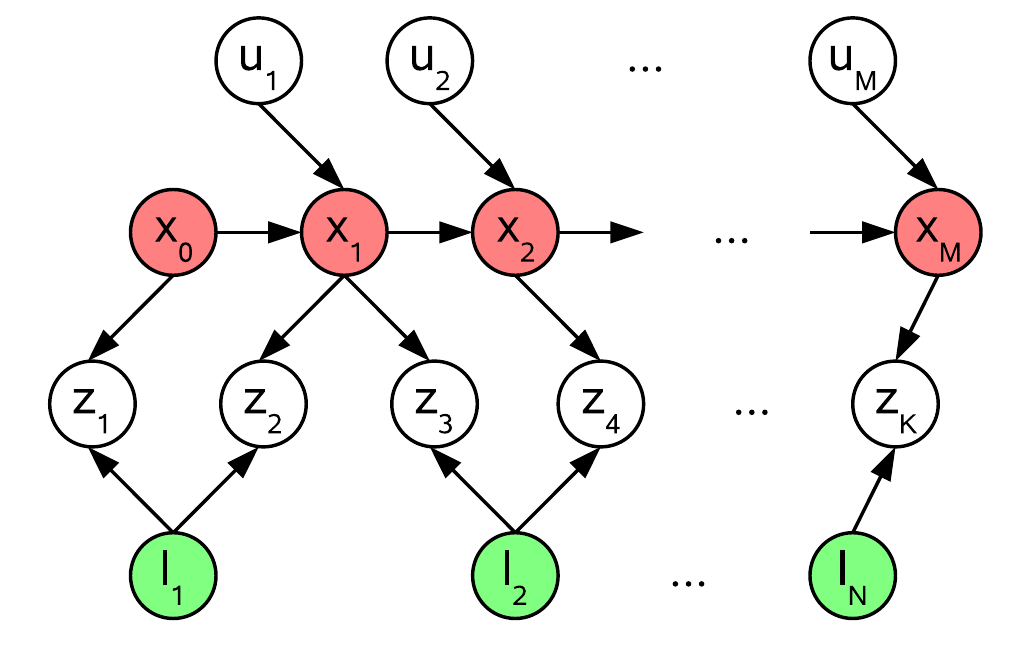
\includegraphics[width=0.4\textwidth]{images/kaess_slam_graph.png}
	\caption{
		SLAM graph with $x_i$ as the robot position at time step $i$. $l_j$ is the $j^{th}$ landmark. $z_k$ is the $k^{th}$ by the robot measured landmark. $u_i$ is the control input at time step $i$ which is for example odometry data \cite{kaess_isam:_2008}. For understanding: At time step $1$ the robot position was $x_1$ and it measured landmark $l_1$ and $l_2$ which can be seen by the measurements $z_2$ and $z_3$. The input from the control unit was $u_1$.
	}
	\label{fig:kaess_slam_graph}
\end{figure}

One large disadvantage is that Kalman filters are only following one hypothesis. For example, when tracking a car at a crossing it could be better to follow the hypothesis, that the car is going straight, but also the hypothesis that the car will turn right or left. When tracking using the Kalman filter, the car could be lost after the crossing. That's where the concept of particle filters was introduced \cite{qun_particle_filter}. In contrast to Kalman filters, particle filters can follow multiple hypotheses. To be exact, each particle can follow one hypothesis.

State-of-the-art SLAM techniques using graph-based approaches. While the robot is moving and making measurements a graph is build up as illustrated in figure \ref{fig:kaess_slam_graph}. With modern graph algorithms the position $x_0, ... , x_n$ can now be estimated. In figure \ref{fig:grisetti_slam_showcase} the performance of those approaches is illustrated.

\begin{figure}[h!]
	\centering
	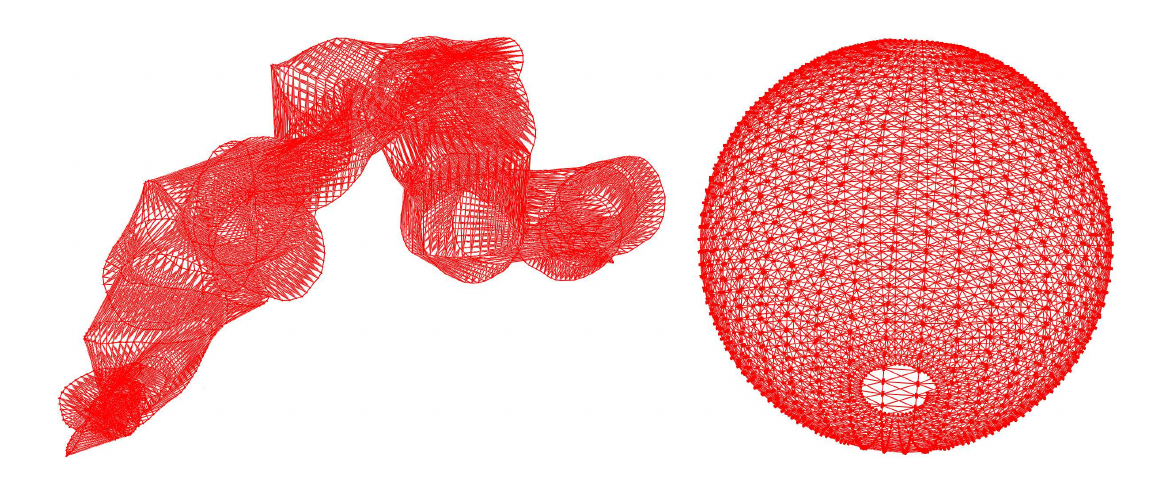
\includegraphics[width=\textwidth]{images/grisetti_slam_showcase.png}
	\caption{
		A showcase of a current state-of-the-art graph-based SLAM approach. Initial position estimation on the left and next to it graph-based SLAM position estimation. The robot was moved in a simulation on the surface of a sphere \cite{grisetti_tutorial_2010}.
	}
	\label{fig:grisetti_slam_showcase}
\end{figure}

When switching from discrete landmarks to continuous functions, these functions need to be approximated within the area of the environment. So it is possible to have values between the measurements which is necessary to improve the position estimation of the actor. When knowing the input space (in this case the environment) but don't want to make any assumptions to the underlying function, Gaussian processes (GP) are the solution \cite{ebden_gaussian_2015}.

Basically, GP are defined by a mean function $m(x) = \mathbb{E}(y(x))$ and a covariance function $k(x_i, x_j) = \mathbb{E}((y(x_i) - m(x_i)) (y(x_j) - m(x_j)))$ also called the kernel. If $m(x) = 0$ the GP are called centered. For the kernel, radial basis functions can be used which means $k(x_i, x_j) = k(||x_i - x_j||)$. Such GP are called radial. One very common radial kernel is the squared exponential kernel \cite{ebden_gaussian_2015}

$$
k(x_i, x_j) = \sigma ^2 \exp 
\begin{pmatrix}
-\frac{(x_i - x_j)^2}{2l^2}
\end{pmatrix}\text{.}
$$

As mentioned before, for SLAM it should be possible to model normally distributed measurements. GP can model normally distributed uncertainty. Assume the noise is normally distributed with variance $\sigma^2_{noise}$. Then measurements can be described as $y_i = f(x_i) + \mathcal{N}(0, \sigma^2_{noise})$. Combining the covariance function with the model of noisy measurements, that will lead to the slightly changed kernel
$$
k(x_i, x_j) = \sigma ^2 \exp 
\begin{pmatrix}
-\frac{(x_i - x_j)^2}{2l^2}
\end{pmatrix}
+ \delta_{ij} \sigma^2_{noise}
$$
where $\delta_{ij}$ is the Kronecker delta. This function is only $1$ when $i=j$ otherwise it is $0$. So, the covariance $k(x_i, x_j)$ is only increased by $\sigma^2_{noise}$ when $i=j$. That means the uncertainty increases for $k(x_i, x_i)$ which are the measurements. Figure \ref{fig:gaussian_process_example} gives an example of GP with and without noisy measurements.

Assume now there are $n$ measurements $y_1, ..., y_n$ taken at $x_1, ..., x_n$. Then the covariance matrix would be
$$
K = \begin{bmatrix}
k(x_1, x_1) & k(x_1, x_2) & \dots & k(x_1, x_n) \\
k(x_2, x_1) & k(x_2, x_2) & \dots & k(x_2, x_n) \\
\vdots & \vdots & \ddots & \vdots \\
k(x_n, x_1) & k(x_n, x_2) & \dots & k(x_n, x_n) \\
\end{bmatrix}\text{.}
$$
Because of GP modeling data from a multivariate normal distribution, $y$ and $y_*$ can be modeled as
$$
\begin{bmatrix}
y \\
y_* \\
\end{bmatrix} 
\sim
\mathcal{N} 
\begin{pmatrix}
0, 
\begin{bmatrix}
K & K_*^T \\
K_* & K_{**} \\
\end{bmatrix}
\end{pmatrix}\text{with}
$$
$$
K_* = [k(x_*, x_1), \dots, k(x_*, x_n)],
$$
$$
K_{**} = k(x_*, x_*)\text{.}
$$
Using the mathematics of multivariate Gaussian distributions, the most likely value of $y_*$ can be calculated by
$$
y_*|y \sim \mathcal{N}(K_*K^{-1}y, K_{**} - K_*K^{-1}K_*^T)
$$
$$
\Rightarrow {y}_* = m(x_*) = K_*K^{-1}y\text{ .}
$$
The derivation of the formula is well explained by Ebden \cite{ebden_gaussian_2015}. Notice that also the variance for $y_*$ is given by
$$
var(y_*) = K_{**} - K_*K^{-1}K_*^T\text{ .}
$$

\begin{figure}[h!]
	\centering	
	\subfloat{{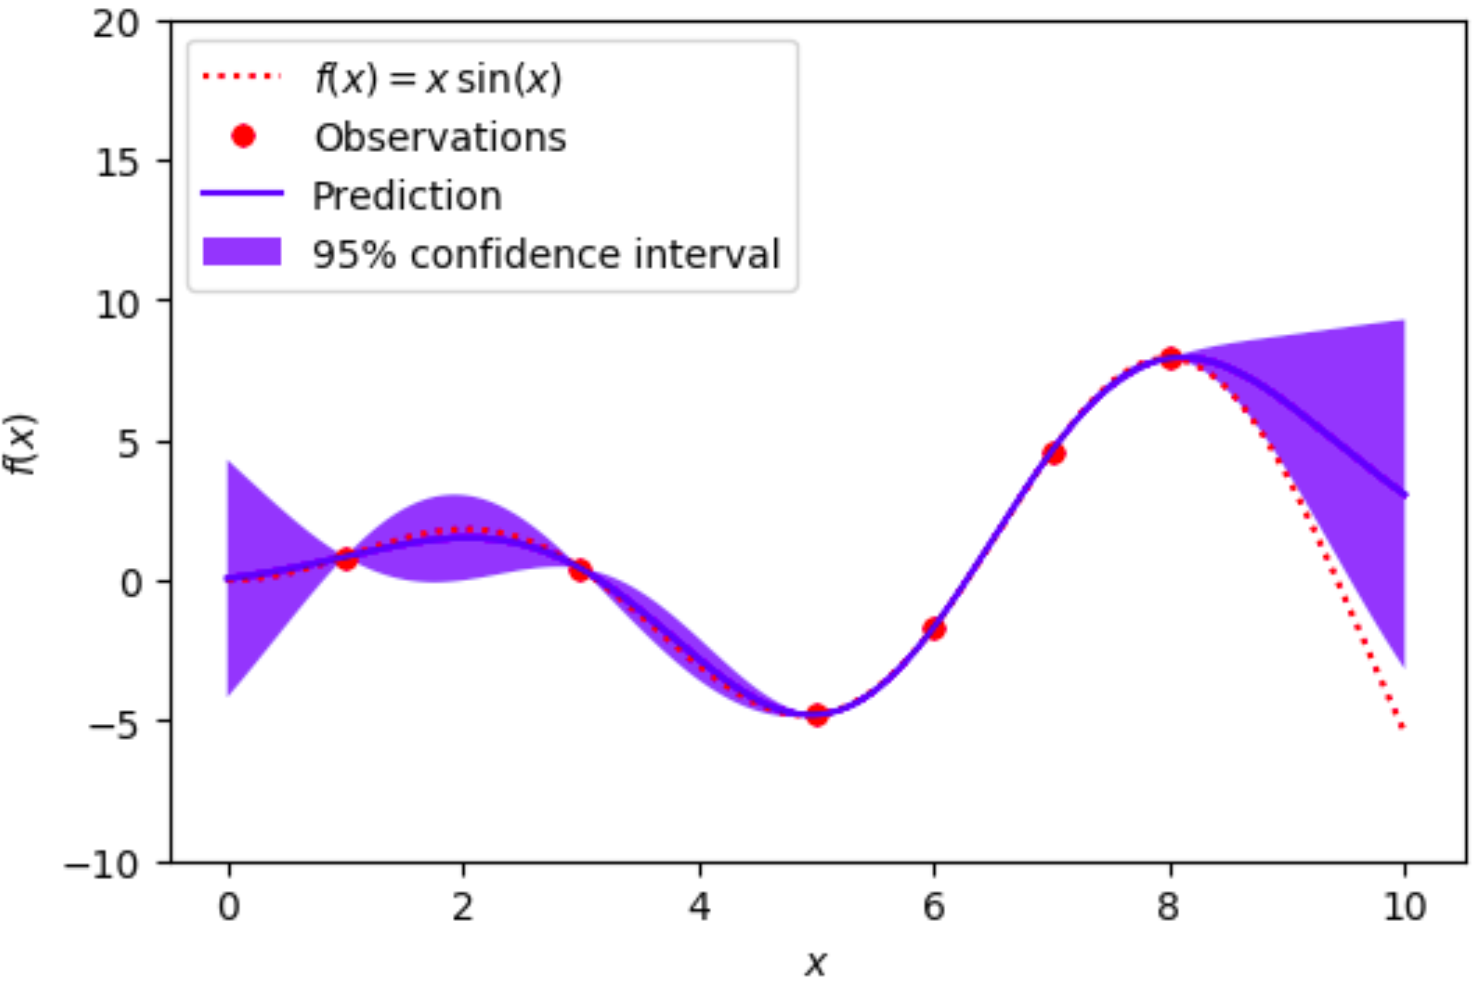
\includegraphics[width=0.5\textwidth]{images/gaussian_process_example1.png} }}
	\subfloat{{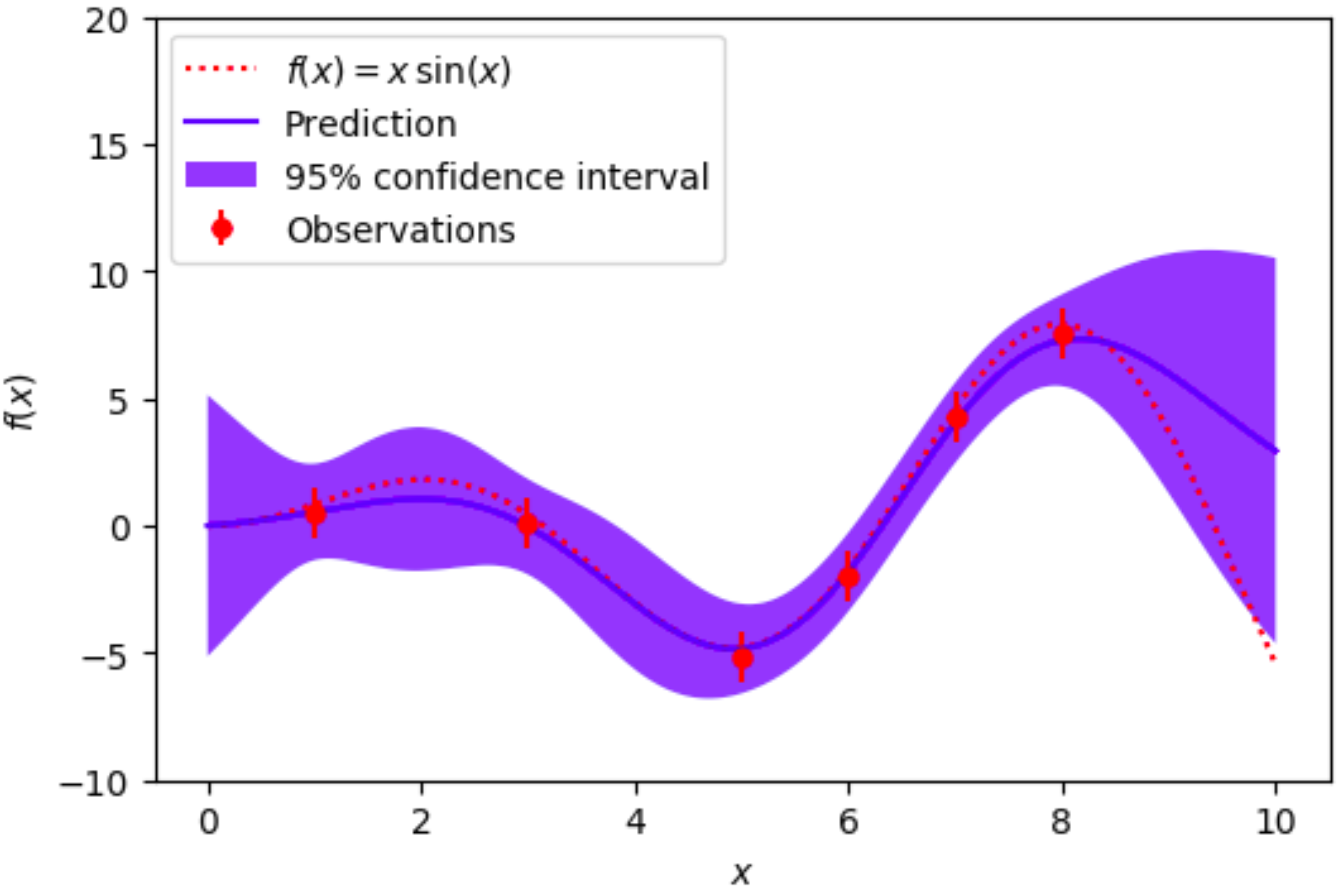
\includegraphics[width=0.5\textwidth]{images/gaussian_process_example2.png} }}
	\caption{
		A plot of two GP regressions with the same measurements $f(x_i)$ but the one at the right has noisy measurements with variance $\sigma_{noise}^2 = 1$. The uncertainty is represented through the confidence interval.
	}
	\label{fig:gaussian_process_example}
\end{figure}

An example of uncertainty in measurements, prediction of $y_*$ and probability of the prediction can be seen in Figure \ref{fig:gaussian_process_example}. Note that for linear increasing number of measurements the size of the covariance matrix rises quadratically and for $y_*$ the inverse of that matrix has to be calculated. So it is computational expensive for large-scale data. There are approaches which facing that problem. Another remark is that the standard GP is not possible to model uncertainty in the input data. So it is not possible to model uncertainty in the position of the robot with GP. 

\section{State of the Art}
\label{chap:stat_of_the_art}

In this Chapter, some recent SLAM approaches based on continuous functions will be presented. It exemplifies what performance current approaches have and on what work this project is based on. 

\subsection{Scalable Magnetic Field SLAM}
\label{sec:scalable_magnetic_slam}

One impressing approach from Kok et al. showing full SLAM in 3D using the magnetic field and GP \cite{kok_scalable_2018}. The magnetic field was approximated with GP and because of performance issues the environment is divided in 3D hexagons as illustrated in figure \ref{fig:kok_example}. So there is a GP for each hexagonal region. This reduces the size of the covariance matrix for each GP and increases performance. 

To approximate the magnetic field, they use a combination of two kernels, the linear and squared exponential kernel and a mean centered around zero \cite{kok_scalable_2018}, that leads to the 
following Gaussian process
$$
GP(0, k_{lin}(x_i, x_j) + k_{se}(x_i, x_j)) \text{ with}
$$
$$
k_{lin}(x_i, x_j) = \sigma_{lin}^2 x_i^T x_j, 
$$
$$
k_{se} = \sigma_{se}^2 \exp 
\begin{pmatrix}
-\frac{||x_i - x_j||^2}{2l^2}
\end{pmatrix}\text{.}
$$

For position estimation, Kok et al. don't use any graph-based approach. Instead, they use a combination of Kalman and particle filter. To update measurements a Kalman filter is used. For predictions in time particle filters are used. A detailed description can be found in their paper \cite{kok_scalable_2018}. Figure \ref{fig:kok_example} demonstrates the performance of their approach. This paper shows vivid what SLAM approaches with continuous functions are capable of.

\begin{figure}[h!]
	\centering
	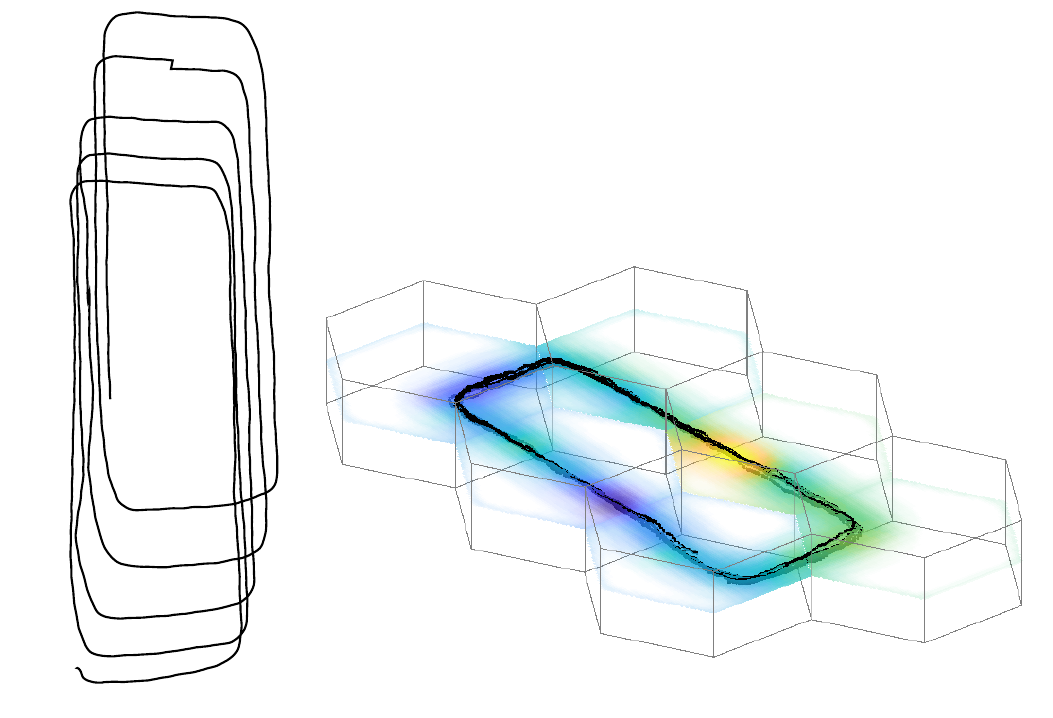
\includegraphics[width=0.8\textwidth]{images/kok_example.png}
	\caption{
		Performance demonstration of the SLAM algorithm by Kok et al. \cite{kok_scalable_2018}. The trajectory on the left shows the odometry data collected by an iPhone 6s and next to it the resulting trajectory with the approximated magnetic field.
	}
	\label{fig:kok_example}
\end{figure}

\newpage
\subsection{Terrain Field SLAM}
\label{sec:terrain_slam}
Another interesting approach from Yu et al. shows which different continuous functions could be used for SLAM \cite{yu_terrain_2018}. In their paper, they described a SLAM algorithm where the continuous function is the vibration caused by the interaction between the robot and the terrain. Their experimental setup and the robot can be seen in figure \ref{fig:yu_setup}.

\begin{figure}[h!]
	\centering
	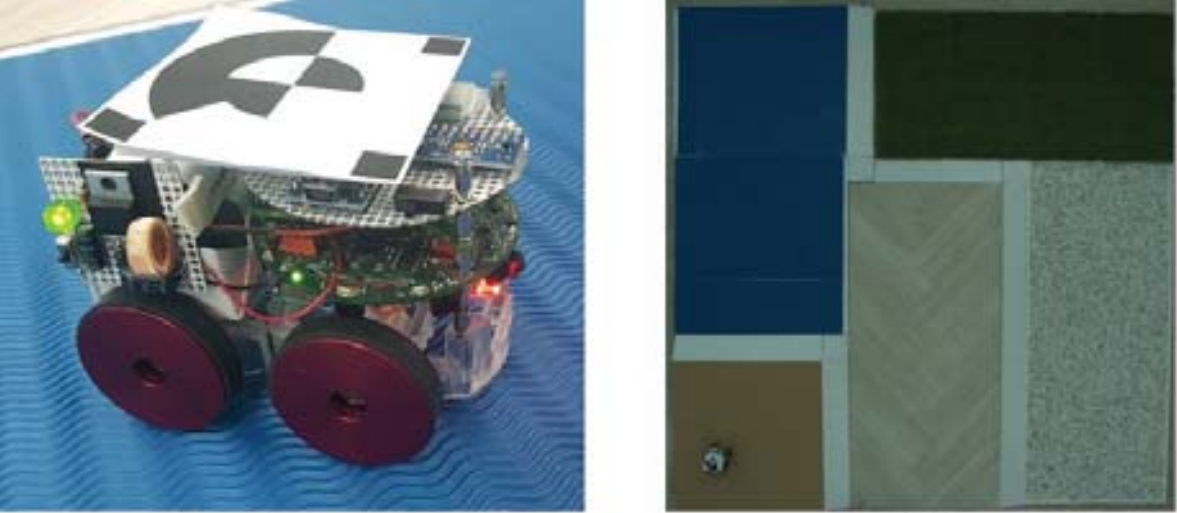
\includegraphics[width=0.8\textwidth]{images/yu_setup.png}
	\caption{
		Illustration of the setup by Yu et al. \cite{yu_terrain_2018}. The mobile robot at the left and
		on the right the environment for the robot to move in. The environment containing
		five different subsurfaces.
	}
	\label{fig:yu_setup}
\end{figure}

Yu et al. also used GP to infer the terrain field. A performance demonstration can be seen in figure \ref{fig:yu_performance}. Even if they don't face the problem of doing SLAM and Gaussian regression on-line and there is a little deviation over time, the results are considerable.


\begin{figure}[h!]
	\centering
	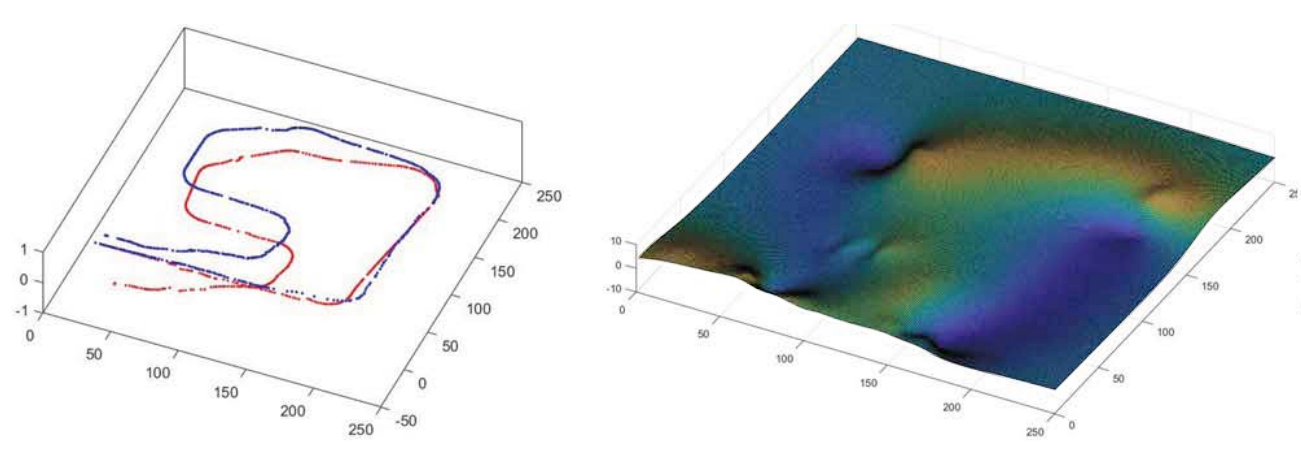
\includegraphics[width=\textwidth]{images/yu_performance.png}
	\caption{
		Performance illustration of the terrain based SLAM approach by Yu et al. \cite{yu_terrain_2018}.
		Robot trajectory (red) on the left and ground truth (blue). Righ shows inferred terrain field.
	}
	\label{fig:yu_performance}
\end{figure}

\subsection{Acoustic SLAM}
\label{sec:acoustic_slam}

When thinking about other potential phenomena for SLAM approaches, acoustic would be a good option. Speakers are cheap and normally a lot of electronic devices have one. Also, acoustic approaches could be used underwater in contrast to camera-based SLAM or the approaches described in Section \ref{sec:scalable_magnetic_slam} and \ref{sec:terrain_slam}.

What nearly all acoustic-based approaches have in common, that they have a prepared environment. Evers et al. in their paper about A-SLAM \cite{evers_aslam_2016} is a good example. They use speakers placed in a room emitting a specific signal and an actor equipped with a microphone array to calculate the incoming directions of the speaker signals. Each speaker acts as a landmark which position has to be estimated so it shouldn't move over time. Although it is a landmark-based approach, it shows what performance an acoustic-based SLAM could have.

\begin{figure}[h!]
	\centering
	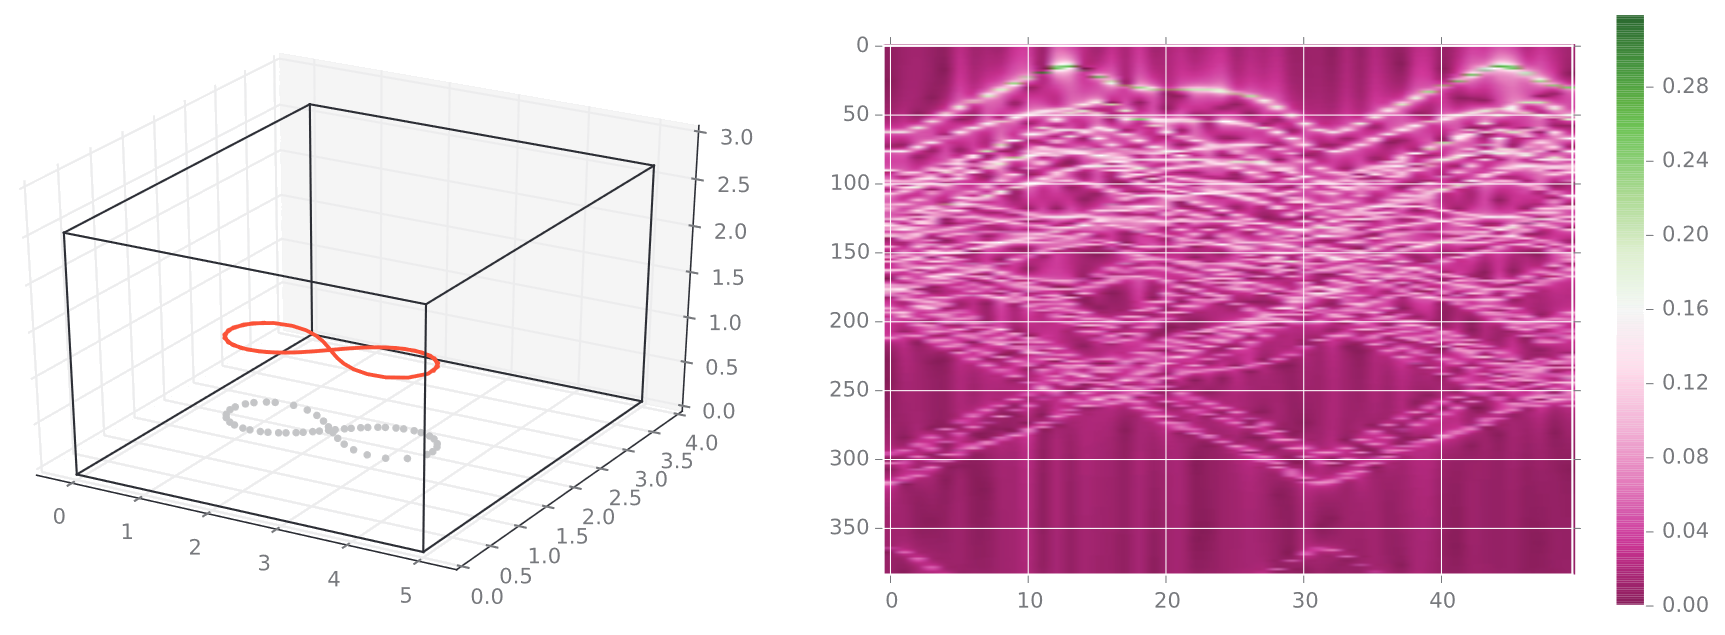
\includegraphics[width=\textwidth]{images/acoustic_slam.png}
	\caption{
		RIR illustration of Dokmanic et al. \cite{dokmanic_roomrecslam_2016}. Left Image shows the trajectory in red of the robot. At the right a plot of the RIR where x-axis is the time and y-axis the RIR.
	}
	\label{fig:dokmanic_roomrecslam}
\end{figure}

There are also acoustic SLAM approaches based on continuous functions. One is from Dokmanic et al. who use the concept of room impulse response (RIR) from room reconstruction for a SLAM approach \cite{dokmanic_roomrecslam_2016}. Therefore he placed a speaker in the room which is sending a specific signal. An actor can now move around and calculate the RIR based on the current position. This RIR is used for SLAM. One thing to point out that in this paper the RIR is a smooth continuous function when the robot is moving and when the robot passes the same point the RIR will be similar (see Figure \ref{fig:dokmanic_roomrecslam}).
